
%% bare_conf.tex
%% V1.3
%% 2007/01/11
%% by Michael Shell
%% See:
%% http://www.michaelshell.org/
%% for current contact information.
%%
%% This is a skeleton file demonstrating the use of IEEEtran.cls
%% (requires IEEEtran.cls version 1.7 or later) with an IEEE conference paper.
%%
%% Support sites:
%% http://www.michaelshell.org/tex/ieeetran/
%% http://www.ctan.org/tex-archive/macros/latex/contrib/IEEEtran/
%% and
%% http://www.ieee.org/

%%*************************************************************************
%% Legal Notice:
%% This code is offered as-is without any warranty either expressed or
%% implied; without even the implied warranty of MERCHANTABILITY or
%% FITNESS FOR A PARTICULAR PURPOSE!
%% User assumes all risk.
%% In no event shall IEEE or any contributor to this code be liable for
%% any damages or losses, including, but not limited to, incidental,
%% consequential, or any other damages, resulting from the use or misuse
%% of any information contained here.
%%
%% All comments are the opinions of their respective authors and are not
%% necessarily endorsed by the IEEE.
%%
%% This work is distributed under the LaTeX Project Public License (LPPL)
%% ( http://www.latex-project.org/ ) version 1.3, and may be freely used,
%% distributed and modified. A copy of the LPPL, version 1.3, is included
%% in the base LaTeX documentation of all distributions of LaTeX released
%% 2003/12/01 or later.
%% Retain all contribution notices and credits.
%% ** Modified files should be clearly indicated as such, including  **
%% ** renaming them and changing author support contact information. **
%%
%% File list of work: IEEEtran.cls, IEEEtran_HOWTO.pdf, bare_adv.tex,
%%                    bare_conf.tex, bare_jrnl.tex, bare_jrnl_compsoc.tex
%%*************************************************************************

% *** Authors should verify (and, if needed, correct) their LaTeX system  ***
% *** with the testflow diagnostic prior to trusting their LaTeX platform ***
% *** with production work. IEEE's font choices can trigger bugs that do  ***
% *** not appear when using other class files.                            ***
% The testflow support page is at:
% http://www.michaelshell.org/tex/testflow/



% Note that the a4paper option is mainly intended so that authors in
% countries using A4 can easily print to A4 and see how their papers will
% look in print - the typesetting of the document will not typically be
% affected with changes in paper size (but the bottom and side margins will).
% Use the testflow package mentioned above to verify correct handling of
% both paper sizes by the user's LaTeX system.
%
% Also note that the "draftcls" or "draftclsnofoot", not "draft", option
% should be used if it is desired that the figures are to be displayed in
% draft mode.
%
\documentclass[10pt, conference, compsocconf, reqno]{IEEEtran}

% Add the compsoc option for Computer Society conferences.
%
% If IEEEtran.cls has not been installed into the LaTeX system files,
% manually specify the path to it like:
% \documentclass[conference]{../sty/IEEEtran}

% Some very useful LaTeX packages include:
% (uncomment the ones you want to load)


% *** MISC UTILITY PACKAGES ***
%
%\usepackage{ifpdf}
% Heiko Oberdiek's ifpdf.sty is very useful if you need conditional
% compilation based on whether the output is pdf or dvi.
% usage:
% \ifpdf
%   % pdf code
% \else
%   % dvi code
% \fi
% The latest version of ifpdf.sty can be obtained from:
% http://www.ctan.org/tex-archive/macros/latex/contrib/oberdiek/
% Also, note that IEEEtran.cls V1.7 and later provides a builtin
% \ifCLASSINFOpdf conditional that works the same way.
% When switching from latex to pdflatex and vice-versa, the compiler may
% have to be run twice to clear warning/error messages.






% *** CITATION PACKAGES ***
%
\usepackage{cite}
% cite.sty was written by Donald Arseneau
% V1.6 and later of IEEEtran pre-defines the format of the cite.sty package
% \cite{} output to follow that of IEEE. Loading the cite package will
% result in citation numbers being automatically sorted and properly
% "compressed/ranged". e.g., [1], [9], [2], [7], [5], [6] without using
% cite.sty will become [1], [2], [5]--[7], [9] using cite.sty. cite.sty's
% \cite will automatically add leading space, if needed. Use cite.sty's
% noadjust option (cite.sty V3.8 and later) if you want to turn this off.
% cite.sty is already installed on most LaTeX systems. Be sure and use
% version 4.0 (2003-05-27) and later if using hyperref.sty. cite.sty does
% not currently provide for hyperlinked citations.
% The latest version can be obtained at:
% http://www.ctan.org/tex-archive/macros/latex/contrib/cite/
% The documentation is contained in the cite.sty file itself.






% *** GRAPHICS RELATED PACKAGES ***
%
\ifCLASSINFOpdf
  \usepackage[pdftex]{graphicx}
  % declare the path(s) where your graphic files are
  \graphicspath{{./eps/}}
  % and their extensions so you won't have to specify these with
  % every instance of \includegraphics
  \DeclareGraphicsExtensions{.pdf,.jpeg,.png}
\else
  % or other class option (dvipsone, dvipdf, if not using dvips). graphicx
  % will default to the driver specified in the system graphics.cfg if no
  % driver is specified.
  % \usepackage[dvips]{graphicx}
  % declare the path(s) where your graphic files are
  % \graphicspath{{../eps/}}
  % and their extensions so you won't have to specify these with
  % every instance of \includegraphics
  % \DeclareGraphicsExtensions{.eps}
\fi
% graphicx was written by David Carlisle and Sebastian Rahtz. It is
% required if you want graphics, photos, etc. graphicx.sty is already
% installed on most LaTeX systems. The latest version and documentation can
% be obtained at:
% http://www.ctan.org/tex-archive/macros/latex/required/graphics/
% Another good source of documentation is "Using Imported Graphics in
% LaTeX2e" by Keith Reckdahl which can be found as epslatex.ps or
% epslatex.pdf at: http://www.ctan.org/tex-archive/info/
%
% latex, and pdflatex in dvi mode, support graphics in encapsulated
% postscript (.eps) format. pdflatex in pdf mode supports graphics
% in .pdf, .jpeg, .png and .mps (metapost) formats. Users should ensure
% that all non-photo figures use a vector format (.eps, .pdf, .mps) and
% not a bitmapped formats (.jpeg, .png). IEEE frowns on bitmapped formats
% which can result in "jaggedy"/blurry rendering of lines and letters as
% well as large increases in file sizes.
%
% You can find documentation about the pdfTeX application at:
% http://www.tug.org/applications/pdftex





% *** MATH PACKAGES ***
%
%\usepackage[cmex10]{amsmath}
% A popular package from the American Mathematical Society that provides
% many useful and powerful commands for dealing with mathematics. If using
% it, be sure to load this package with the cmex10 option to ensure that
% only type 1 fonts will utilized at all point sizes. Without this option,
% it is possible that some math symbols, particularly those within
% footnotes, will be rendered in bitmap form which will result in a
% document that can not be IEEE Xplore compliant!
%
% Also, note that the amsmath package sets \interdisplaylinepenalty to 10000
% thus preventing page breaks from occurring within multiline equations. Use:
%\interdisplaylinepenalty=2500
% after loading amsmath to restore such page breaks as IEEEtran.cls normally
% does. amsmath.sty is already installed on most LaTeX systems. The latest
% version and documentation can be obtained at:
% http://www.ctan.org/tex-archive/macros/latex/required/amslatex/math/


\usepackage{listings}
\usepackage{color}

\definecolor{dkgreen}{rgb}{0,0.6,0}
\definecolor{gray}{rgb}{0.5,0.5,0.5}
\definecolor{mauve}{rgb}{0.58,0,0.82}

\lstset{ %
  language=C,                % the language of the code
  basicstyle=\footnotesize\ttfamily,           % the size of the fonts that are used for the code
  numbers=right,                   % where to put the line-numbers
  numberstyle=\tiny\color{gray},  % the style that is used for the line-numbers
  stepnumber=0,                   % the step between two line-numbers. If it's 1, each line
                                  % will be numbered
  numbersep=0pt,                  % how far the line-numbers are from the code
  %backgroundcolor=\color{white},      % choose the background color. You must add \usepackage{color}
  showspaces=false,               % show spaces adding particular underscores
  showstringspaces=false,         % underline spaces within strings
  showtabs=false,                 % show tabs within strings adding particular underscores
  %frame=single,                   % adds a frame around the code
  rulecolor=\color{black},        % if not set, the frame-color may be changed on line-breaks within not-black text (e.g. commens (green here))
  tabsize=2,                      % sets default tabsize to 2 spaces
  captionpos=b,                   % sets the caption-position to bottom
  breaklines=true,                % sets automatic line breaking
  breakatwhitespace=false,        % sets if automatic breaks should only happen at whitespace
  title=\lstname,                   % show the filename of files included with \lstinputlisting;
                                  % also try caption instead of title
  keywordstyle=\bfseries,          % keyword style
  commentstyle=\color{dkgreen},       % comment style
  stringstyle=\color{mauve},         % string literal style
  escapeinside={\%*}{*)},            % if you want to add LaTeX within your code
  morekeywords={*,...}               % if you want to add more keywords to the set
}


% *** SPECIALIZED LIST PACKAGES ***
%
\usepackage{algpseudocode}
\usepackage{algorithm}
%\usepackage{algorithmic}
%\usepackage{algorithmicx}
% algorithmic.sty was written by Peter Williams and Rogerio Brito.
% This package provides an algorithmic environment fo describing algorithms.
% You can use the algorithmic environment in-text or within a figure
% environment to provide for a floating algorithm. Do NOT use the algorithm
% floating environment provided by algorithm.sty (by the same authors) or
% algorithm2e.sty (by Christophe Fiorio) as IEEE does not use dedicated
% algorithm float types and packages that provide these will not provide
% correct IEEE style captions. The latest version and documentation of
% algorithmic.sty can be obtained at:
% http://www.ctan.org/tex-archive/macros/latex/contrib/algorithms/
% There is also a support site at:
% http://algorithms.berlios.de/index.html
% Also of interest may be the (relatively newer and more customizable)
% algorithmicx.sty package by Szasz Janos:
% http://www.ctan.org/tex-archive/macros/latex/contrib/algorithmicx/




% *** ALIGNMENT PACKAGES ***
%
%\usepackage{array}
% Frank Mittelbach's and David Carlisle's array.sty patches and improves
% the standard LaTeX2e array and tabular environments to provide better
% appearance and additional user controls. As the default LaTeX2e table
% generation code is lacking to the point of almost being broken with
% respect to the quality of the end results, all users are strongly
% advised to use an enhanced (at the very least that provided by array.sty)
% set of table tools. array.sty is already installed on most systems. The
% latest version and documentation can be obtained at:
% http://www.ctan.org/tex-archive/macros/latex/required/tools/


\usepackage{mdwmath}
\usepackage{mdwtab}
% Also highly recommended is Mark Wooding's extremely powerful MDW tools,
% especially mdwmath.sty and mdwtab.sty which are used to format equations
% and tables, respectively. The MDWtools set is already installed on most
% LaTeX systems. The lastest version and documentation is available at:
% http://www.ctan.org/tex-archive/macros/latex/contrib/mdwtools/


% IEEEtran contains the IEEEeqnarray family of commands that can be used to
% generate multiline equations as well as matrices, tables, etc., of high
% quality.


%\usepackage{eqparbox}
% Also of notable interest is Scott Pakin's eqparbox package for creating
% (automatically sized) equal width boxes - aka "natural width parboxes".
% Available at:
% http://www.ctan.org/tex-archive/macros/latex/contrib/eqparbox/





% *** SUBFIGURE PACKAGES ***
\usepackage[tight,footnotesize]{subfigure}
% subfigure.sty was written by Steven Douglas Cochran. This package makes it
% easy to put subfigures in your figures. e.g., "Figure 1a and 1b". For IEEE
% work, it is a good idea to load it with the tight package option to reduce
% the amount of white space around the subfigures. subfigure.sty is already
% installed on most LaTeX systems. The latest version and documentation can
% be obtained at:
% http://www.ctan.org/tex-archive/obsolete/macros/latex/contrib/subfigure/
% subfigure.sty has been superceeded by subfig.sty.



\usepackage[font=small,center,belowskip=-10pt,aboveskip=5pt]{caption}
%\usepackage[font=footnotesize]{subfig}
% subfig.sty, also written by Steven Douglas Cochran, is the modern
% replacement for subfigure.sty. However, subfig.sty requires and
% automatically loads Axel Sommerfeldt's caption.sty which will override
% IEEEtran.cls handling of captions and this will result in nonIEEE style
% figure/table captions. To prevent this problem, be sure and preload
% caption.sty with its "caption=false" package option. This is will preserve
% IEEEtran.cls handing of captions. Version 1.3 (2005/06/28) and later
% (recommended due to many improvements over 1.2) of subfig.sty supports
% the caption=false option directly:
%\usepackage[caption=false,font=footnotesize]{subfig}

%
% The latest version and documentation can be obtained at:
% http://www.ctan.org/tex-archive/macros/latex/contrib/subfig/
% The latest version and documentation of caption.sty can be obtained at:
% http://www.ctan.org/tex-archive/macros/latex/contrib/caption/




% *** FLOAT PACKAGES ***
%
%\usepackage{fixltx2e}
% fixltx2e, the successor to the earlier fix2col.sty, was written by
% Frank Mittelbach and David Carlisle. This package corrects a few problems
% in the LaTeX2e kernel, the most notable of which is that in current
% LaTeX2e releases, the ordering of single and double column floats is not
% guaranteed to be preserved. Thus, an unpatched LaTeX2e can allow a
% single column figure to be placed prior to an earlier double column
% figure. The latest version and documentation can be found at:
% http://www.ctan.org/tex-archive/macros/latex/base/



%\usepackage{stfloats}
% stfloats.sty was written by Sigitas Tolusis. This package gives LaTeX2e
% the ability to do double column floats at the bottom of the page as well
% as the top. (e.g., "\begin{figure*}[!b]" is not normally possible in
% LaTeX2e). It also provides a command:
%\fnbelowfloat
% to enable the placement of footnotes below bottom floats (the standard
% LaTeX2e kernel puts them above bottom floats). This is an invasive package
% which rewrites many portions of the LaTeX2e float routines. It may not work
% with other packages that modify the LaTeX2e float routines. The latest
% version and documentation can be obtained at:
% http://www.ctan.org/tex-archive/macros/latex/contrib/sttools/
% Documentation is contained in the stfloats.sty comments as well as in the
% presfull.pdf file. Do not use the stfloats baselinefloat ability as IEEE
% does not allow \baselineskip to stretch. Authors submitting work to the
% IEEE should note that IEEE rarely uses double column equations and
% that authors should try to avoid such use. Do not be tempted to use the
% cuted.sty or midfloat.sty packages (also by Sigitas Tolusis) as IEEE does
% not format its papers in such ways.





% *** PDF, URL AND HYPERLINK PACKAGES ***
%
%\usepackage{url}
% url.sty was written by Donald Arseneau. It provides better support for
% handling and breaking URLs. url.sty is already installed on most LaTeX
% systems. The latest version can be obtained at:
% http://www.ctan.org/tex-archive/macros/latex/contrib/misc/
% Read the url.sty source comments for usage information. Basically,
% \url{my_url_here}.





% *** Do not adjust lengths that control margins, column widths, etc. ***
% *** Do not use packages that alter fonts (such as pslatex).         ***
% There should be no need to do such things with IEEEtran.cls V1.6 and later.
% (Unless specifically asked to do so by the journal or conference you plan
% to submit to, of course. )

\newcommand{\INDSTATE}[1][1]{\STATE\hspace{#1\algorithmicindent}}
\newcommand{\comment}[1]{}

%squeeze

\renewcommand{\arraystretch}{1}

\renewcommand\floatpagefraction{.9}
\renewcommand\topfraction{.9}
\renewcommand\bottomfraction{.9}
\renewcommand\textfraction{.1}
\setcounter{totalnumber}{50}
\setcounter{topnumber}{50}
\setcounter{bottomnumber}{50}

\raggedbottom

\addtolength{\floatsep}{-5mm}
\addtolength{\textfloatsep}{-3mm}
%~ \addtolength{\intextsep}{-2mm}
\addtolength{\dbltextfloatsep}{-2mm}
\addtolength{\dblfloatsep}{-1mm}
\addtolength{\abovecaptionskip}{-1mm}
\addtolength{\belowcaptionskip}{-1mm}
\addtolength{\abovedisplayskip}{-3mm}
\addtolength{\belowdisplayskip}{-3mm}
\addtolength{\arraycolsep}{-1mm}

\let\oldthebibliography=\thebibliography
\let\endoldthebibliography=\endthebibliography
\renewenvironment{thebibliography}[1]{%
  \begin{oldthebibliography}{#1}%
    \setlength{\parskip}{0.2ex}%
    \setlength{\itemsep}{0.2ex}%
}%
{%
  \end{oldthebibliography}%
}

\captionsetup{justification=centering}

% correct bad hyphenation here
\hyphenation{op-tical net-works semi-conduc-tor}

\begin{document}
%
% paper title
% can use linebreaks \\ within to get better formatting as desired
\title{A parallel runtime framework for communication intensive stream applications}

% author names and affiliations
% use a multiple column layout for up to three different
% affiliations
\author{\IEEEauthorblockN{Servesh Muralidharan\IEEEauthorrefmark{2},
Kevin Casey\IEEEauthorrefmark{4}
and
David Gregg\IEEEauthorrefmark{2}}
\IEEEauthorblockA{\IEEEauthorrefmark{2}School of Computer Science and Statistics,
Trinity College Dublin, Dublin 2, Ireland\\
Email: muralis@scss.tcd.ie, David.Gregg@cs.tcd.ie }
\IEEEauthorblockA{\IEEEauthorrefmark{4}School of Computing, Dublin City University, Glasnevin, Dublin 9, Ireland\\
Email: Kevin.Casey@computing.dcu.ie}
}
%~
%~ \author{\IEEEauthorblockN{Servesh Muralidharan}
%~ \IEEEauthorblockA{School of Computer Science and\\Statistics\\
%~ Trinity College Dublin\\
%~ Dublin 2, Ireland\\
%~ Email: muralis@tcd.ie}
%~ \and
%~ \IEEEauthorblockN{David Gregg}
%~ \IEEEauthorblockA{School of Computer Science and\\Statistics\\
%~ Trinity College Dublin\\
%~ Dublin 2, Ireland\\
%~ Email: David.Gregg@cs.tcd.ie}}

% conference papers do not typically use \thanks and this command
% is locked out in conference mode. If really needed, such as for
% the acknowledgment of grants, issue a \IEEEoverridecommandlockouts
% after \documentclass

% for over three affiliations, or if they all won't fit within the width
% of the page, use this alternative format:
%
%\author{\IEEEauthorblockN{Michael Shell\IEEEauthorrefmark{1},
%Homer Simpson\IEEEauthorrefmark{2},
%James Kirk\IEEEauthorrefmark{3},
%Montgomery Scott\IEEEauthorrefmark{3} and
%Eldon Tyrell\IEEEauthorrefmark{4}}
%\IEEEauthorblockA{\IEEEauthorrefmark{1}School of Electrical and Computer Engineering\\
%Georgia Institute of Technology,
%Atlanta, Georgia 30332--0250\\ Email: see http://www.michaelshell.org/contact.html}
%\IEEEauthorblockA{\IEEEauthorrefmark{2}Twentieth Century Fox, Springfield, USA\\
%Email: homer@thesimpsons.com}
%\IEEEauthorblockA{\IEEEauthorrefmark{3}Starfleet Academy, San Francisco, California 96678-2391\\
%Telephone: (800) 555--1212, Fax: (888) 555--1212}
%\IEEEauthorblockA{\IEEEauthorrefmark{4}Tyrell Inc., 123 Replicant Street, Los Angeles, California 90210--4321}}


% use for special paper notices
%\IEEEspecialpapernotice{(Invited Paper)}


% make the title area
\maketitle


\begin{abstract}
%\boldmath
Stream applications are often limited in their performance by their underlying communication system. A typical implementation relies on the operating system to handle the majority of network operations. In such cases, the communication stack, which was not designed to handle such tremendous amounts of data, acts as a bottleneck and restricts the performance of the application.

In this paper, we propose a parallel runtime framework that integrates the communication operations with stream applications, and provides a common parallel processing engine that can execute both the communication and computation operations in parallel on multicore processors.

Our runtime system does this by using a series of communication filters that transform the data from the application to packets suitable for transmission. These communication filters are built using system software that allows direct access to network hardware. We also utilize the ability of the modern network controller to classify packets onto multiple hardware queues by integrating it with the communication filter. Using this, our runtime framework is able to construct a unified stream graph based on the application graph provided. This, when used with a static schedule based on a given architecture, can process the data streams in parallel.

We are able to parallelize stream applications and achieve speedups of more than a factor of eight in all the applications we tested. The results show that our system scales to as many as 24 parallel processes on a multicore computer, and achieves speedups of more than a factor of ten in some cases compared to sequential implementations.

\end{abstract}
% IEEEtran.cls defaults to using nonbold math in the Abstract.
% This preserves the distinction between vectors and scalars. However,
% if the conference you are submitting to favors bold math in the abstract,
% then you can use LaTeX's standard command \boldmath at the very start
% of the abstract to achieve this. Many IEEE journals/conferences frown on
% math in the abstract anyway.

% no keywords


% For peer review papers, you can put extra information on the cover
% page as needed:
% \ifCLASSOPTIONpeerreview
% \begin{center} \bfseries EDICS Category: 3-BBND \end{center}
% \fi
%
% For peerreview papers, this IEEEtran command inserts a page break and
% creates the second title. It will be ignored for other modes.
\IEEEpeerreviewmaketitle
%Kevin - vertical spacing % Servesh - Fixed it on global command
%\setlength{\textfloatsep}{15pt}
\section{Motivation}

Applications that follow a streaming model~\cite{Thies:2002:SLS:647478.727935,Halbwachs91thesynchronous,Stephens95asurvey,muthukrishnan2005data}
are expressed as a network of \textit{filters} connected by communication
\textit{channels}. Tokens of data flow along the communication channels
between filters. Each filter consumes on one or more \textit{streams}
of data from its input channels, and produces streams of data on its
ouput channels. For applications that fit the model well, stream processing
can greatly reduce the working memory required. Since the data flows through
a sequence of filters in a pipelined style, it is often possible to
operate on a relatively small window of the data at any given time,
thereby making it possible to operate on conceptually infinite
data streams.

Traditionally, the stream processing model was used primarily
for signal processing type applications, where the application
processes a continuous stream of signal inputs. For example,
many video processing applications are modelled as a set of
image filters operating on a stream of video frame, where the
entire video may be hundreds of gigabytes in size, but the
processing can be done with just a few frames at a time.
However, in more recent years it has been found that the stream
model is highly suitable for many applications that process
very large data sets, in the order of terabytes or even larger.
Applications such as financial trading
systems~\cite{agarwal2009faster},
database systems~\cite{Golab03datastream},
network data analysis~\cite{Gilbert01quicksand:quick,Sullivan:1998:TSM:1268256.1268258} are a few examples that follow the streaming model and also operate on very large data sets.

Stream processing is highly suited to multicore and parallel
computing, because the filters can typically execute in parallel.
Smaller stream applications often achieve high levels of parallelism
on multicore machines.  However, as the stream processing model
is used to address larger data processing problems, more computational
resources are needed, and a common solution is to distribute the
filters across a number of machines.
In such cases, the applications are typically limited by the
traditional communication
~\cite{Wu:2007:PPB:1323954.1323957,Wu:2007:PAL:1227865.1228021,Dobrescu09routebricks:exploiting,Han:2010:PGS:1851275.1851207,Kohler2000}.
The main reason for this is that these systems have limited support for operating on
parallel streams and are burdened by abstraction layers that provide
compatibility for non-streaming applications.

Several high speed networks~\cite{fredj2011survey} exist that could handle such communication requirements but these require expensive hardware and specialized programming skills. Commodity network adapters based on 10-gigabit ethernet (10GbE) are a comparatively cheaper alternative and are being widely deployed in clusters and grids in data centers. Previous research\cite{Romanow03anoverview,Feng:2003:OEN:1048935.1050200} has been done on optimizing ethernet for improving communication in such cases. However, they do not use many of the features provided by modern day network adapters such as hardware queues, flow control, etc., Also, they do not focus specifically on streaming applications and hence making it difficult to utilize them properly.

\section{Contribution}

In this paper we propose a parallel runtime framework for building stream applications that are bound by very large communication. A simple framework is used, where the filters are described as \textit{actors} and the application is represented by connecting such \textit{actors} into a directed acyclic graph (DAG). Then our framework is used to establish, (1)the communication system that allows these \textit{actors} to send and receive data across each other and (2)the computation system that executes these tasks in parallel on a given multicore system. The main contributions can be described as,

\begin{enumerate}
\item A parallel multi point communication layer, which provides the ability for stream actors to communicate across the network
\item An execution system that can run the given data-parallel filters on the multicore system
\item The utilization of network hardware features such as queues and flow control to support stream applications.

\end{enumerate}

\comment{
We focus on integrating the packet processing and application tasks into a single graph and using this to extract data parallelism. The developer describes their program as a graph of \textit{filters}. Each actor consumes one or more \textit{tokens} of data, which may be simple data such as integers, or more complex data such as packets, arrays, or objects and produces one or more tokens. The framework can be used to automatically map the application over multiple parallel cores, and interface with the \texttt{netmap} APIs \cite{Rizzo:2012:RNI:2090147.2103536} for accessing data through the network buffers.

The system can be divided into three main parts:

\begin{itemize}
\item A subsystem for interfacing with the network hardware through the \texttt{netmap} APIs to send and receive data from the application in user space without going through the operating system. (Section \ref{ppio})
\item Given a graph that represents the workload to be performed by the application, we construct and integrate the packet processing operations represented as a directed acyclic graph (DAG) to it. (Section \ref{ppe})
\item A run-time system that executes these tasks in parallel and explicitly schedules them on the multicore processor. (Section \ref{ppt})
\end{itemize}
}

% Even though we integrate the system with the application, the techniques for extracting parallelism from the application is not in scope of this paper. The application is considered to be in a streaming model and the tasks corresponding to the various functions are considered to be parallel in nature.

\comment{
With the continuing improvement of multicore and many-core architectures, it is becoming essential to improve the processing speeds of packet operations along with those of the application in order to scale performance.
}
\comment{
When performing packet processing operations for communication intensive stream applications, a major challenge is the high levels of performance required. These applications process large numbers of data streams in real time.  If the communication system cannot keep up with the rate at which packets arrive, then they must be dropped or remain unprocessed.
}

\section{Introduction}

Our main objective is to optimize performance of streaming applications by first, providing a specialized communication link between the filters and second, extracting data-parallel actors and executing them in parallel. Stream applications usually consists of stateless and stateful filters. Stateful filters are those that are depedendent on the previous execution which makes it difficult to replicate them. Stateless filters do not pose such limitations and can be freely replicated based on the available data streams. In this paper, we focus on extracting data parallelism based on stateless filters and streams. Example operations of such an application are represented in the stream graph shown in Figure \ref{fig1}. All the filters used in this application are essentially stateless filters. This application operates by performing encryption on the data that matches predefined rules like file names, access level of user, etc., otherwise it performs compression. Due to the nature of such stream applications, it is possible to replicate and distribute the filters across different CPUs. We are particularly interested in a scenario where groups of networked servers are used to perform these kind of stream operations by distributing data streams over multiple nodes.

\begin{figure}[ht]
\centering
\subfigure
{
	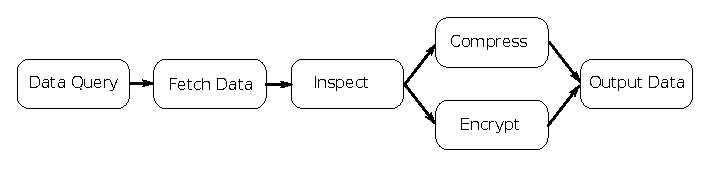
\includegraphics[width=3.5in]{ip-data-proc}
}

\subfigure
{
	\includegraphics[width=3in]{op-data-proc}
}
\caption{Sample stream application}
\label{fig1}
\end{figure}

The main challenge that arises in such a situation is how best to address the intensive computational and communication demands of such applications. Two important features enable us to tackle this challenge in our framework. Firstly, the operations of both the application and the network are designed to be stateless filters. Secondly, communication techniques are employed that would enable multicore processors to perform operations related to computation and communication in parallel.

In building a framework for such applications on general purpose computers, we can exploit two hardware features that could allow for dramatically improved performance, namely multicore processors and multi queue network controllers. By using the multiple queues makes it possible to the communication in parallel and by using the multiple cores, the filters from the stream application can be executed concurrently.

A major bottleneck for communication on general purpose computers is the overhead of the operating system's network stack. In particular, for applications that run as user processes, data must be copied between OS kernel space and user space. Previous research uses alternate mechanisms to access data from the network hardware directly to overcome this problem\cite{Dobrescu09routebricks:exploiting}\cite{Han:2010:PGS:1851275.1851207}\cite{Kohler2000}. Most of these use modern network hardware in combination with specialized system software that allows direct access to hardware-controlled packet queues, dramatically reducing overheads and improving performance. However, constructing stream applications that use these features is difficult. Furthermore, many stream applications have a very specific communication pattern, typically operating on a \textit{flow}, which is a specific \textit{stream} between two filters. Data in a \textit{stream} must be processed sequentially, whereas different \textit{flows} can often be processed in parallel.

Newer network hardware have introduced mechanisms for separating arriving data into multiple queues, where data that belong to the same \textit{flow} are\comment{ guaranteed to be} placed in the same queue\cite{micro2008} \cite{intel2010}. We can utilize this feature to operate on \textit{flows} by processing each of the queues in parallel. However, building applications that can use this feature directly is a challenging task because it requires explicit parallel programming and interaction with low-level network interfaces. Previous research~\cite{Dobrescu09routebricks:exploiting,Han:2010:PGS:1851275.1851207} that focuses on improving the performance of network applications in such a manner shows the complexity involved in building such a system.

\comment{We parallelize both the application and packet operations to gain significant improvement in performance.}

In our framework, we use a more elegant approach. We define a runtime framework that provides pre-built communication filters. In order to implement a stream application such as that shown in Figure~\ref{fig1}, all we need to do is define the computation filters and connect them in the framework to the pre-built communication filters. On execution, our runtime framework is able to replicate the stateless filters and the communication filters onto the different multiple cores, thereby executing the operations belonging to different \textit{flows} in parallel.

\comment{
 parallel processing framework that could be leveraged on multicore processors and multi queue network controllers to achieve efficient communication. The performance of multicore processors continues to dramatically improve the capability of commodity hardware, thus making it possible to meet the computational demand of such applications. In addition, multi queue network interface controllers, designed to handle multiple streams of data, help achieve the necessary communication performance.

An important part of our system is the tasks related to packet processing in protocols such as UDP, IP, etc., We utilize the modular router, Click, for these packet processing tasks. Click is a tool that includes a library of elements which is used in building flexible, re-configurable and modular software routers \cite{Kohler2000}. It offers a high-performance platform that is flexible for rapid development of newer network protocols. An improved version known as SMP Click supports thread-based parallel processing of network related tasks\cite{Chen:2001:FCP:647055.759948}. Until recently, Click's performance in the user space was inferior to its kernel space equivalent. This is mainly due to its extensive use of polling driver in the kernel space that was not possible in user space. Netmap I/O\cite{Rizzo:2012:RNI:2090147.2103536} provides a set of APIs that can directly access the packets from the NIC and was used to improve Click's user space performance. Although other other user space packet-access APIs could be used \cite{Rizzo:2012:RNI:2090147.2103536} \cite{1564468} \cite{Krasnyansky}, the simpler construction of \texttt{netmap} was more suitable to adapt to our framework.
}

Section \ref{dppl} represents the design principles that we follow to conceptualize our framework. Section \ref{imple} describes the implementation details used in the construction of the system. In section \ref{ppe}, we discuss the challenges in using a system consisting of execution engines to manage the work. \comment{The extent to which we extract parallelism ranges, not only to the packet tasks, but also to the low level access of data I/O to the network interface hardware through custom additions to the \texttt{netmap}.} Finally in section \ref{app-const}, we present a simple stream application constructed from operations such as compression and encryption and evaluate our framework.

\section{Design Principles}
\label{dppl}

The design of a high-level programming framework that integrates packet processing tasks into the application requires overcoming several challenges. \comment{The entire system is driven by the extent to which parallelism can be extracted. Some of the techniques that can be applied to the packet processing tasks can be used for the tasks related to the application.} In this section, we describe these challenges and the principles that are used to address them. \comment{We focus on the methodologies related to the packet processing tasks and the parallel processing engine itself.}

\subsection{Communication filters}

\comment{Understanding the set of packet processing tasks associated with the application is essential to performing them in parallel.} We use a graph-based representation of filters related to packet processing to determine the dependencies involved for the different stages and to determine the relation with the different tasks of the application. This graph contains the stages through which the data associated with the application is transformed into network packets and vice versa. It shows which of the tasks can be performed in parallel with those of the application, and highlights those that have a data dependency on a specific task in the application. The graph also enables optimizations based on specific characteristics of the application or the architecture used for execution. Figure \ref{fig2} shows a simple graph representing User Datagram Protocol (UDP) packet generation.

\begin{figure}[ht]
\centering
\includegraphics[width=3.5in]{pack-op}
\caption{Simplified UDP packet construction}
\label{fig2}
\end{figure}

\subsection{Userspace communication}

For a communication system to be integrated with an application, it is necessary to have an efficient mechanism for reading and writing packets to and from the NIC without interacting with the operating system. Rapid data access here is crucial for the extraction of data parallelism at later stages. We use a number of techniques to support this rapid data access.\comment{In using the techniques described below we exploit the modern NIC architecture to its full potential.}

\subsubsection{Handling Multiple Hardware Queues}

The development of virtualization and improved network flow handling has led to hardware-level multi queue support in NICs. During transmission, concurrent writes to different queues are possible, enabling multiple processes to send data simultaneously. During reception, the NIC classifies each packet onto one of the receive queues in a technique known as Receive Side Scaling (RSS)\cite{micro2008} \cite{intel2010}. This technique uses the header information or tuples to classify packets onto different hardware queues. Multi queue support can handle several streams of data in parallel and it is exploited extensively in our framework for this reason. By offloading the classification of packets to the NIC, we remove any overhead associated with packet classification in the application. We can also use these hardware queues as a means of balancing the workload across different threads by controlling the number of queues that each thread handles. \comment{Since different processes can access these transmit and receive queues, concurrent access to data is possible.}

\subsubsection{Flow based communication}

A common technique known as \texttt{batching} is used to boost the performance of network applications, where several packets are combined and operated upon together, thus reducing the overhead of I/O operations. In our framework, batching is utilized in a form where the number of packets in a batch is varied based on the available space in the hardware queue. This number reflects the amount of data we are able to process before issuing hardware synchronization calls and forms an important means by which we reduce the usage of system calls.

\subsubsection{Reduction of Per Packet System Calls}

System calls are required in order to synchronize data between the NIC hardware and the buffer memory used for intermediate storage of data. Previous work describes the overhead associated with per-packet system calls and provides mechanisms for overcoming this overhead\cite{1564468}\cite{Han:2010:PGS:1851275.1851207}\cite{Rizzo:2012:RNI:2090147.2103536}.

We employ an \textit{adaptive scheme} described in section \ref{ppio} that utilizes this strategy of reducing per-packet system calls. Our framework balances the system calls based on the communication rate and application processing speed. The transmission and reception are handled differently to optimize the usage of system calls in each of the cases independently. During transmission, we issue system calls to synchronize the available buffer space based on the rate at which we transmit data. This prevents degradation in latency for larger packets and improves performance for smaller packets. During reception of packets, the system reads packets at the rate at which it is able to process them.

\subsection{Computation filters}

\comment{Computation filters represents the operations associated . The subset of the application that we are interested in parallelizing is the stream processing component.} In stream processing model, the communication flow between tasks is well-defined. \comment{This is usually represented by a synchronous data flow graph (SDF).} The filters associated with the computation can be connected to the communication filters in the same directed acyclic graph (DAG) used to represent the application. \comment{The packet processing tasks operate on packets and the application tasks operate on the data. Since we focus more on parallel packet processing, optimizations in relation to the application graph are not discussed. It is assumed that a static version of the application graph is available and we focus more on executing these tasks in parallel with the packet processing tasks.} The computation filters are designed by the user and are programmed into the runtime framework which already provides the communication filters.

\subsection{Integration}

\comment{The sequence of tasks that can be executed in parallel is determined at this stage. The integration stage is used to combine the application graph and the packet processing graph into a larger graph that unifies and represents the overall operations. The dependency relations identified earlier are used in establishing links between the graphs. We determine the sequence of tasks that can be executed in parallel from both the application task graph and packet processing graph. The combined set of tasks is then used by the parallel processing engine.}

This stage essentially connects the corresponding communication filter to the computation filter defined earlier. Based on the stream graph that is provided, the necessary communication filters are added. This also determines the unique \textit{flows} that exists between the filters and is used later to replicate and execute them in parallel.

\subsection{Parallel Processing Engine}

Two important aspects that the parallel processing engine must address is the scheduling of filters and the balancing of the load across the available resources. The parallel processing engine consists of collaborating processes which are bound to specific CPUs and act as engines to execute the workload. Based on their requirements and the available resources, filters are scheduled across these execution engines. We assume a static schedule of the filters onto the given multiple cores is provided for execution. \comment{In this manner, the workload can be distributed flexibly.}

\section{Implementation}
\label{imple}

\comment{Most extant stream applications depend on the OS for their communication tasks.}In commodity systems, the interaction with the OS for network operations is a necessary abstraction to handle multiple applications. However, in the case of specialized servers which cater to specific applications, it would be beneficial to interact directly with the network device. Moreover, in the case of intensive network traffic, the OS could act as a bottleneck due to the overhead associated with data flowing through the kernel before being transmitted through the network device\cite{Wu:2007:PPB:1323954.1323957}\cite{Wu:2007:PAL:1227865.1228021}. Eliminating this would be possible, either by executing the application in the kernel space (which could compromise stability of the system), or by using an interface for accessing the NIC buffers from user space. The latter approach is supported by several interfaces such as \texttt{netmap} \cite{Rizzo:2012:RNI:2090147.2103536}, PF\_RING DNA \cite{1564468}, UIO-IXGBE \cite{Krasnyansky}, etc., Even though these interfaces support user space packet access, they lack the ability to be invoked in a efficient manner by the application. More specifically, they do not have any way of optimizing the rate of processing, lacking, for example, the concept of flows for application tasks. These application tasks are represented as computation filters similar to those described in figure~\ref{fig1}. The lack of support for interacting with these interfaces in order to read and write data in parallel from concurrent processes or threads adds to the problem. Also, since the application is now responsible for handling network packets, it has to perform the additional operations that would otherwise be carried out by the OS.

Our framework provides support for sending and receiving data in parallel over the NIC from user space and a common parallel execution engine that supports both computation and communication filters.

\subsection{Parallel communication interface}
\label{ppio}
The parallel communication interface, when combined with the computation filters, provides concurrent communication for the application threads or processes over the network. To do this, two important requirements have to be met. Firstly, access to network data from user space should be provided, which can be read from and written to in parallel. Secondly, it should be possible to integrate this with the computation by providing the necessary communication filters that can perform packet operations. The ability to choose communication filters allows the flexibility in the choice of communication protocol.

\subsubsection{Userspace data access}
If applications are executed in kernel space for accessing data from network devices directly would lead to scenario where the operating system can become unstable. Instead, previous researchers \cite{Rizzo:2012:RNI:2090147.2103536}, \cite{1564468}, \cite{Krasnyansky}, etc., propose access to network buffers from user space. We use \texttt{netmap} APIs \cite{Rizzo:2012:RNI:2090147.2103536} to access data from the network buffers. \texttt{Netmap} uses a set of ring buffers in kernel space and user space to export the network hardware buffer's memory region. This enables applications in user space to directly access the network hardware. It also prevents applications from accessing memory outside valid regions by checking the limits of the ring buffer. Packets can be written to the buffers when space is available, and an \textit{ioctl} call to the driver enables the network controller to send the data. A \textit{poll} interface is implemented on the memory region mapped in user space to check when new packets are available. On reading or writing packets, the available space is updated.

We leverage the availability of multiple hardware queues present in modern NICs to read and write data concurrently. \texttt{Netmap}, by default, supports assigning each hardware queue to an individual application process or thread. However, in order to allow for more efficient communication in the framework, we required the ability to assign more than one queue to a particular thread or process. Our modifications to \texttt{netmap}'s hardware queue assignment API allow our framework to balance the amount of packets handled by each process by varying the number of queues assigned to it.

During testing, it was found that it was essential to have control over the rate at which system calls were issued with respect to the amount of data being transferred. Frequent system calls hamper bandwidth and limit the peak performance of the application. To tackle this, we propose the following algorithms for reading and writing data from the hardware queues using the \texttt{Netmap} APIs. These algorithms are designed to provide the following features,

\begin{itemize}

\item Provide batching of packets based on available space on hardware rings
\item Reduce the usage of system calls such as \textit{ioctl} and \textit {poll}
\item Provide mechanisms for handling multiple queues through the application.

\end{itemize}

\comment{By minimizing the synchronizations with the hardware rings, we essentially limit the system calls issued and consequently improve the overall system performance.}










Algorithms \ref{s_pack} and \ref{r_pack} use a batch update for sending and receiving packets based on the rate at which data flows through the interface. This is done by maintaining a data structure that has information about the hardware rings, updating it on a periodic basis. Once a fixed amount of space is determined, we update this on our local structure. We then continue to read or write data from the hardware ring, but update the actual limits and position on our local structure. When we have used up the space that was allocated, we update the hardware ring with the changes. In cases where the application is generating sparse traffic, it is possible to frequently update the ring in order to maintain a consistent latency in transmission. Multi queue support is provided by managing the process of selecting the ring to send or receive based on an application determined function. The $f(n)$ present in Algorithm \ref{s_pack} line \ref{s_pack_param} and Algorithm \ref{r_pack} line \ref{r_pack_param} represents this. Choosing a random queue ($f(n)=X \sim U([0,n])$ n=no of queues) has proven to be effective in our experiments, but if an application requires a specific flow to be maintained, a different function here could provide that support. This would be helpful in cases where the data operations are more predictable, or if the transactions seem to follow a specific pattern. The $threshold$ specified in Algorithm \ref{r_pack} line \ref{r_pack_thres} is determined for each application based on the rate at which it is able to process data. By issuing the system calls such as \textit{ioctl} and \textit{poll} only when required, and effectively handling the multiple queues, we are able to achieve improved performance.


\setlength{\textfloatsep}{0pt}


\begin{algorithm}[h]
\caption{To send packets}
\label{s_pack}
\begin{algorithmic}[1]

\State \textbf{struct} $ring[ n ]$\textbf{\{}
\State \Comment{Stores information about hardware rings}
\State \Comment{ $ n \gets \ $tx\ rings\ assigned\ to\ thread}
\State \  \  $avb$, available space
\State \  \  $curr$, current position
\State \  \  $limit$, total space \ \textbf{\}}

\Function{send\_data\_mqueue}{Ring $f(n)$, Data $packet$}
\While{$!success$}
	\State $i \gets f( n ) $ \label{s_pack_param}
	\State $success = $ \texttt{SEND\_DATA}($ i, packet $)
\EndWhile
\EndFunction
\Function{send\_data}{Ring $i$, Data $packet$}
\If{ $ring[ i ].avb > 0$ }
	\State $hw\_ring[ i ].slot( ring[ i ].curr ) \gets packet$
	\State $ring[ n ].avb \gets ring[ i ].avb - 1$
	\State $ring[ i ].curr++$
	\If{ $ring[ i ].avb == 0$ }
		\State $hw\_ring[ i ].avb \ -=\ ring[ i ].limit$
		\State $hw\_ring[ i ].curr \gets ring[ i ].curr$
	\EndIf
	\State \textbf{return} $success$
\EndIf

\State \textbf{\textit{issue ioctl and poll}}
\State $ring[ i ].avb \gets hw\_ring[ i ].avb$
\State $ring[ i ].limit \gets hw\_ring[ i ].avb$
\EndFunction

\end{algorithmic}
\end{algorithm}

\subsubsection{Packet processing operations}

Packet processing operations consist of converting the raw data that the application provides into network packets suitable for transmission. Since the application tasks are represented as a set of operations on a data stream, we include these operations as stages through which the data flows through to get transformed into data packets. This is done by representing these operations as communication filters pre-built into our runtime system. Integrating them with the application task graph makes it easier to extract parallelism later in the execution engine. Several user space libraries exist that perform packet related processing operations like libnids \cite{libnids}, lwip \cite{Dunkels01designand}, Click \cite{Kohler2000} etc. Since our application is targeted at a closed environment, we chose the Click modular router due to its flexibility and vast library of elements. Our current framework supports the UDP protocol but Click's modular infrastructure makes it easy to support more complex ones. \comment{Indeed, stream applications with more complex protocols would benefit even more from the framework due to the parallelizing of these complex tasks.}

Each of the elements in Click contain a virtual function which is called from the previous element it is attached to. It was necessary to overcome the limitation of Click's infrastructure where elements are constructed based on dynamically initialized objects and virtual functions. This was required due to the need to eliminate the overhead associated with the dynamic construction of the objects and virtual functions, and also to allow for optimizing the task graph along with these operations. To achieve these goals, our framework provides a simple support structure to allow Click elements to be imported and to be integrated with applications.
\begin{algorithm}[h]
\caption{To receive packets}
\label{r_pack}
\begin{algorithmic}[1]

\State \textbf{struct} $ring[ n ]$\textbf{\{}
\State \Comment{Stores information about hardware rings}
\State \Comment{ $ n \gets \ $rx\ rings\ assigned\ to\ thread}
\State \  \  $avb$, available packets
\State \  \  $curr$, current position
\State \  \  $limit$, total packets \ \textbf{\}}

\Function{receive\_data\_mqueue}{Ring $f(n)$}
\While{$!packet$}
	\State $i \gets f( n ) $ \label{r_pack_param}
	\State $packet =$ \texttt{RECEIVE\_DATA}(Ring $i$)
\EndWhile
\EndFunction

\Function{receive\_data}{Ring $i$}
\If{ $ring[ i ].avb > 0$ }
	\State $packet \gets hw\_ring[ i ].slot( ring[ i ].curr ) $
	\State $ring[ i ].avb \gets ring[ i ].avb - 1$
	\State $ring[ i ].curr++$
	\If{ $ring[ i ].avb < threshold$ } \label{r_pack_thres}
		\State $hw\_ring[ i ].avb -= ring[ i ].( limit - avb)$
		\State $hw\_ring[ i ].curr \gets ring[ i ].curr$
		\State $ring[ i ].avb \gets hw\_ring[ i ].avb$
		\State $ring[ i ].limit \gets hw\_ring[ i ].avb$
	\EndIf
	\State \textbf{return} $packet$
\EndIf

\State \textbf{\textit{issue ioctl and poll}}
\State $ring[ i ].avb \gets hw\_ring[ i ].avb$
\State $ring[ i ].limit \gets hw\_ring[ i ].avb$
\EndFunction

\end{algorithmic}
\end{algorithm}
\subsection{Parallel Processing Engine}

After defining the communication filters by means of \texttt{Click}'s infrastructure and access to network hardware through \texttt{netmap}'s APIs, we integrate these filters with the application tasks. The results is a complete stream graph that does both the computation and communication operations. The next logical step is executing these filters in parallel by exploiting data parallelism. Packet streams are inherently operable in a data parallel fashion i.e. it is possible to operate on two different streams simultaneously. \comment{Since the application tasks depend on the data packets, they could also be executed in parallel. So from the integrated graph constructed by combining the application and packet processing operations, it becomes possible to extract data parallelism by operating on different data streams simultaneously. By executing different components, representing distinct operations on the data streams, it is also possible to exploit task parallelism.}

\subsubsection{Execution engine}
\label{ppe}

The execution engine consists of a set of processes and threads that the work is scheduled upon in order to be executed. When implementing threads to execute code which consist of system calls such as \textit{malloc(), ioctl(), poll(),} etc., we found a performance degradation, even when the threads are completely independent. To support the lightweight style of threads, the OS implements most of the locking mechanisms for system calls from threads. Previous research such as \cite{Lever:2000:MPM:1267724.1267780} \cite{Dice:2002:MLM:773039.512451} \cite{Michael:2004:SLD:996893.996848} shows the degradation in performance due to the usage of \textit{malloc()} in threads. Since our framework has to deal with system calls and issue them in parallel, we use \textit{unix process} to perform the tasks concurrently. We do this by using Message Passing Interface (MPI) \cite{TheMPIForum:1993:MMP:169627.169855} to construct a set of processes that is scheduled onto the different CPUs on a multicore system.

In order to prevent unwanted process migration due to the OS scheduler, we specify \textit{affinity} of the MPI processes to particular CPU cores. This prevents each process from being executed on a different CPU other than that specified. This makes the processes act as execution engines, running on each of the cores on which we schedule the operations that are to be performed. Previous research \cite{Salehi:1996:EAS:234766.234769}\cite{1409136} highlights the importance of affinity in network sensitive applications. Next, by utilizing our \textit{Parallel communication interface}~(\ref{ppio}), we specify the hardware queues each of these processes handle. \comment{Initially we divide the queues evenly among the different processes we create, but later during execution we could modify the allocation based on the application operations scheduled on them. Our modifications to \texttt{netmap}'s hardware queue assignment API can help us here in redistributing the queues to different processes.} By using MPI's \texttt{send} and \texttt{receive} inter-process communication calls to handle communication between execution engines located at each CPU, it is possible to modify the attributes of the process such as CPUs assigned or number of NIC queues handled, and even the operations the processes were initially assigned.

\subsubsection{Parallel processing of computation filters}
\label{ppt}

Once we have scheduled our execution engines on the physical system, the next step is to execute the stream graph for different \textit{flows}. To extract data parallelism, we replicate the stream graph onto multiple execution engines. This ensures operations on the same \textit{flow} are performed on the same CPU, thereby using local cache. By making sure that data belonging to a specific \textit{flow} always end up in the same execution engine, we only perform operations conforming to that stream of data. \comment{We use the ability of modern NICs to classify packets onto different queues, based on their attributes.}


\comment{
\lstset{language=C,caption={Packet Payload Modification Function},label=payload_sub}
\begin{lstlisting}
bool payload_copy( const void *payload_data, uint32_t length )
{
    uint32_t headroom = _data - _head;
    uint32_t tailroom = _end - _tail;
    uint32_t orig_length = _tail - _data;
    uint32_t n = length + headroom + tailroom;
    if( n < min_buffer_length )
    {
        tailroom = min_buffer_length - length - headroom;
        n = min_buffer_length;
    }
    _data = _head + headroom;
    _tail = _data + length;
    if( payload_data )
        memcpy( _data, payload_data, length );
    return true;
}
\end{lstlisting}
}

\comment{In order to replicate the task graph we had to overcome some restrictions. First was to ensure that there was no intricate data dependency between different data streams. Although Click's library of elements are designed to be executed in parallel \cite{Chen:2001:FCP:647055.759948}, they are more oriented towards serial execution. Hence we had to ensure the code present in the elements were thread-safe. One important modification we had to perform was in Click's packet library. By default, Click destroys and recreates the packet's internal storage buffer by reallocating memory space, an expensive operation. In order to avoid this, we allocate a packet with a large static buffer and copy the data to be modified on it. We then modify the pointers that determine the header and data addresses, based on the required packet length. \comment{This is done by using a simple sub-routine shown in Listing \ref{payload_sub} that we added to the packet library.} Although this addition incurs the overhead of a copy operation, it avoids performing invalid and dangerous memory operations directly on the network hardware queue's buffer.

Click's packet library also provides a mechanism to take ownership of a specific address and pass a destructor to be called when the packet is killed. To prevent corruption of memory mapped from the hardware queue by the application tasks, we use the above mechanism to copy the data before modifying it. In generating the application graph as a sequence of operations, it also makes it possible to run different graphs on each individual execution engine. MPI communication is used to schedule the application and packet operations on the processes representing the execution engines. Furthermore, we use it to also perform explicit data sharing between tasks in the application that require it.}

\section{Experimental Evaluation}

In order to evaluate our framework, we test the scalability and the performance speedup on a multicore system for an application that is constructed with the framework. Using two generic operations: compression and encryption, we build simple stream applications. We then measure the performance improvement as we increase the number of execution engines dedicated to the application.

\subsection{Hardware Setup}

The evaluation system consists of two servers connected directly to each other. Each server consists of two Intel Xeon 5600 hexacore HT in a dual socket configuration with 24GB DDR3 memory. In total there is 2 Processors x 6 Cores x 2 HT = 24 CPUs in each server. These servers are connected using Intel 8299EB 10Gbe adapters over directly attached twin-axial cables. The adapters are located in the PCI Express x8 slot to provide required bandwidth for the network cards. This forms a closed connection between two servers and limits the influence of external devices such as switches or routers on data transmission.

Each application is constructed in two parts, one a source of data and the other a sink. We measure the overall time it takes for application task operations, communication operations, and the time to send from the source and receive at the sink. This is done for different packet sizes and applications. Then we plot the speedup achieved in each of the cases over the serial version where we have a single sender and receiver operating on the multiple queues. This is the baseline in our experiments and is similar to how the application would behave if it were implemented using just direct access to the network hardware.

The Intel 82599EB is restricted to 16 queues when using Receive Side Scaling (RSS). This limited the maximum amount of processes at the sink to be 16, even though 24 CPUs were available. The source is not affected by this limitation and can use all the 24 CPUs available, along with 24 hardware transmission queues. Overall, we require at least one hardware queue mapped to each of our processes or execution engines. \comment{We also ensure that each of the processes are bound to a particular CPU by issuing affinity calls to the OS to ensure that they are not migrated between different cores.}

\subsection{Application Construction}
\label{app-const}

In order to evaluate our framework, distinct operations were required that would be suitable for a streaming framework. Since compression and encryption applications are relatively common, we chose two applications composed from these operations. The stream graph that represents both these applications is shown in fig \ref{fig-app-graph}. UDP is used to send the data between source and sink.

\begin{figure}[htb]
\centering
\includegraphics[width=3.5in]{enc-dec}
\caption{ Integrated Task Graph  }
\label{fig-app-graph}
\end{figure}

Both applications are constructed similarly. Data sizes of 1.28GB and 2.56GB are selected as the workload for the compression and encryption applications respectively. The OpenSSL library is used for encryption/decryption and zlib is used for compression/decompression operations. Each application consists of a data generation phase, then data is compressed or encrypted depending on the application. Packet operations are performed after the data is generated. The stream consisting of packets is then sent over the network using multiple queues. The sink side performs the reverse of these operations. Once data is received, packet operations are performed to extract the payload, followed by decompression or decryption to retrieve the original data. These are representative of some of the typical operations that would be involved in a much more complex application. \comment{Choosing to compare these simple operations avoids any extraneous factors that may be present in a more complex application.}Use of these simpler stream applications enables us to evaluate the performance of our framework and not that of any optimizations specific to the application.

\begin{figure*}[tb]
\centering
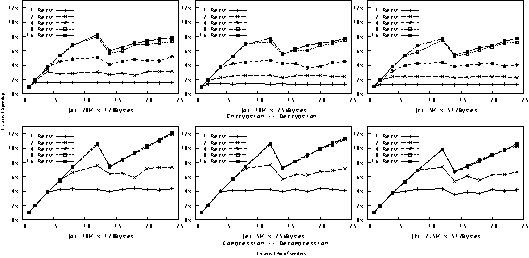
\includegraphics[width=7in]{result}
\caption{Performance Speedup; (a),(b),(c) - Application A. Encryption; (d),(e),(f) - Application B. Compression;\\ \newline Speedup based on time in takes to compute a fixed workload for different number of source and sink processes\\ \newline and for varying packet sizes over a single source and sink are shown above}
\label{fig-res}
\end{figure*}

\section{Results}
\label{results}
It can be seen in Figure \ref{fig-res} that there is considerable difference in the way each of the operations scale. Three distinct observations can be made from the results.

One is that, from fig\ref{fig-res}.(d,e,f), we note that compression requires more work than decompression, whereas from fig\ref{fig-res}.(a,b,c) encryption and decryption are more balanced. This is evident from the continued speedup obtained from up to 4 senders in the case of compression/decompression. Only a slight asymmetry can be seen in the encryption/decryption case, where adding more senders than receivers only yields a slight increase in performance. In this case, the likely explanation is support for AES instructions in the architecture, making decryption a marginally easier task. In general though, the performance here only improves by increasing both the number of senders and receivers simultaneously. Even from these preliminary results, it is clear that the optimal sender/receiver balance varies from application to application and highlights the need for effective load-balancing.

Packet size also impacts performance as seen in fig\ref{fig-res}.(d,e,f). The compression operation is influenced more than that of the encryption application. There is a speedup of 12x in fig\ref{fig-res}.(d) with smaller packets and 10x in fig\ref{fig-res}.(f) with larger packets. This discrepancy appears to be greater in cases where there is a large number of senders and a high number of receivers. A possible explanation for this relates to the CPU utilization on the faster receivers. With large packet sizes, they are more likely to block waiting for data to be streamed from the slower senders. Smaller packets allow the work to be distributed more evenly among the available receivers. In the encryption application, there is not as much asymmetry and packet size does not matter as much. The fact that packet size impacts applications differently suggests that it is essential to incorporate dynamic packet-size selection into the framework itself.\comment{ to respond to the unique requirements of each application.}

From fig\ref{fig-res}(a,b,c,d,e,f), a drop in speedup is apparent when employing 12 senders or more. The most likely explanation for this is the influence of the NUMA architecture \cite{Awasthi:2010:HPO:1854273.1854314}. The 12 sender point is when all the cores of a particular CPU are utilized and moved onto a different socket. This causes issues in relation to cache locality and the limitation of the network controller to receive data through the PCI-E bus from more than one CPU. Despite these NUMA architecture issues, once the initial drop is overcome, the application continues to scale and eventually attain better performance in most cases.

In summary, it can be seen that the framework scales well for different workloads, can handle both computations and communication, and can operate on them in parallel. We see that we can achieve a speedup $10\times$ for compression and $12\times$ for encryption sample stream application respectively on the architecture consisting of two nodes of 24 logical cores each. In some cases, the framework can be improved by having a greater degree of control over the fine grained parallelism within the execution engines. This can be achieved by introducing pipeline stages for different operations.

\comment{Results also suggest where efforts should be made in developing the framework further. Until now, the focus has been on deploying the execution engines in order to execute stream applications and to enable optimal communication between separate nodes.}

\comment{Future work will address some of the opportunities presented by these execution engines and the collaboration between them.}

Since we work with a static schedule provided by the user in executing the applications. Dynamic load balancing is likely to be the most benificial addition to the framework in terms of performance of the stream applications built using it. It is also possible to add the capability to dynamically adjust the number of network queues allocated to each core as stream application requirements change over time. Finally, as seen in Figure~\ref{fig-res}, being able to adjust packet sizes dynamically to an optimal value for each network link, dependant on the stream application, would also be a useful addition to the framework.

\section{Related Work}

Stream programming languages such as StreamIt~\cite{Thies:2002:SLS:647478.727935}, LUSTRE~\cite{Halbwachs91thesynchronous} and extensions such as Carpenter et al.~\cite{Carpenter:2007:SMD:1776200.1776217}, Buck et al.~\cite{Buck:2004:BGS:1015706.1015800} target stream applications, but the focus is more on parallelizing the computations related to the application alone on the multicore system unlike our runtime framework which also parallelizes communication operations.

MPICH-G2~\cite{Karonis02mpich-g2:a} targets large grid networks and applications written using the MPI programming model, unlike our focus on the streaming model. Moreover, we do not employ any of the MPI communication primitives provided to handle streaming data. Instead we use our own fast runtime system to communicate data between the filters in the stream graph across systems.

Wagner et al.~\cite{5160944} propose a stream processing framework that completely utilizes the MPI library. They make use of MPI groups and communicators to improve the flexibility of the MPI library to support stream-processing. Their approach employs a library using MPI primitives to construct their stream-processing system and relies on the underlying abstraction layer to communicate over any network the MPI library supports. Our runtime framework is designed to provide a low overhead, parallel communication framework by directly utilizing the network link.

Mancini et al.~\cite{5493465} propose a hybrid approach of Stream and MPI programming models and use a whole MPI program as building block in a stream application to improve processing speeds of computational units in hetrogeneous computational systems.

While we use MPI to execute the computation filters, our runtime framework employs a direct and parallel communication interface for the actual transmission and reception of data between filters. This is the key feature that enables us to parallelize the communication along with the computation for a given streaming application, which is essential in improving its performance.

\comment{
Several prior researchers \cite{Dobrescu09routebricks:exploiting}\cite{Han:2010:PGS:1851275.1851207}\cite{Wang:2009:PPN:1542275.1542307}\cite{springerlink:10.1007/s11227-011-0579-3} have worked on using commodity multicore processors to perform network operations.

Dobrescu et al.\cite{Dobrescu09routebricks:exploiting} shows the performance improvement achieved in the construction of software routers by distributing related operations over multiple servers.

Han et al. \cite{Han:2010:PGS:1851275.1851207} perform tasks related to high performance packet processing on commodity hardware using GPUs. They have developed a novel framework known as PacketShader that can do packet processing in user space by exploiting the massively-parallel architecture of GPUs.

Wang et al. \cite{Wang:2009:PPN:1542275.1542307} constructs a high performance connection-affinity based lock-free multicore network processing system that claims to achieve multiple Gbps network processing speed for complex tasks.

Egi et al.\cite{springerlink:10.1007/s11227-011-0579-3} shows techniques on parallelizing network operations on multicore architectures by defining principles that consider multiple resources and not just the CPU alone.
}

\comment{
All of these applications are more focused on operating as a network application and primarily focus on parallelizing packet operations. In our work even though a part of it involves parallelizing network operations, the objective of this research is to provide support for parallelizing stream application and distributing their workloads over multiple systems. This also requires optimizing the underlying network operations by parallelizing it.

\texttt{Netmap} \cite{Rizzo:2012:RNI:2090147.2103536}, provides the APIs to access the hardware queue's buffer in user space by means of memory mapped rings. It implements an intermediate ring in kernel space that is used to synchronize the data from the user space to that of hardware queues in the NIC.

The Click modular router \cite{Kohler2000} is an extensively used tool for the construction of software routers using general purpose hardware and provides a comprehensive infrastructure to support this. SMP Click \cite{Chen:2001:FCP:647055.759948} is an improved version, which supports parallel processing of these software routers using threads. Click implements its own mechanism and polling driver in kernel space to access packets, bypassing the OS's network infrastructure.
}

\comment{
In order to send data the programmer calls \textit{poll} on the tx ring in user space and writes to it when space is available. Then he calls \textit{ioctl} to synchronize the data with the kernel ring and transmit the data. To receive the packets \textit{poll} is again called on the rx ring in user space but this time to check for new data and after reading it, he issues \textit{ioctl} to let the driver know that packet has been read and space can be re used.


, our framework uses techniques as described in Section \ref{imple} to integrate them with the application and access them in parallel from different application processes. Also, while some of click's \cite{Kohler2000} elements are used to provide support for packet processing operations, in our framework we use it for doing some of application's network tasks alone. Due to this we modified a subset of click's elements in order to support our system.


 In our framework we target a different category of stream applications such as data mining, real time image analysis, etc., which tend to compute on large amounts of data. In order to improve overall performance in such cases, the operations are distributed over multiple systems. Our framework provides an easier methodology to construct such an application while managing both the parallelizing and communication operations.

Our framework provides the necessary functionality to target communication intensive stream applications. We focus on improving the overall performance of such an application by integrating the network and application operations. We do this by providing a high-level programming framework that can be used to construct these applications, which can extract parallelism and improve communication performance. Using this it would be possible to develop stream applications that could be distributed over multiple systems and using our framework it would be possible to handle the highly intensive communication between them.}

\section{Conclusions}
In this paper we have proposed a parallel runtime framework that can integrate communication and computational operations in stream applications and perform both types of operation in parallel.

Our algorithms for sending and receiving data implicitly perform batching and reduce the usage of system calls, and we combine this with \texttt{netmap} APIs to minimize the interaction with the OS. This allows communication performance in our framework to better scale with the number of available processors. Instead of performing the communication operations separately in the OS, by integrating them within the stream application\comment{using Click's elements within our infrastructure,}, we are able to construct a unified stream graph that represents the entire application, including computation and communication filters. Using this, we are able to parallelize the stream applications and achieve speedups of more than a factor of eight in all the applications we tested.

By integrating these features into a runtime framework, the system of multiple queues, parallel communication and computation are entirely hidden from the programmer, who merely specifies a standard stream graph for computation alone. This frees the programmer from the onerous task of dealing with the implementation of the substantial communication requirements that result from the distribution of stream applications across multiple systems.

The results show that our system scales to as many as 24 parallel processes on a multicore computer, and achieves speedups of more than a factor of ten in some cases compared to sequential implementations.

% An example of a floating figure using the graphicx package.
% Note that \label must occur AFTER (or within) \caption.
% For figures, \caption should occur after the \includegraphics.
% Note that IEEEtran v1.7 and later has special internal code that
% is designed to preserve the operation of \label within \caption
% even when the captionsoff option is in effect. However, because
% of issues like this, it may be the safest practice to put all your
% \label just after \caption rather than within \caption{}.
%
% Reminder: the "draftcls" or "draftclsnofoot", not "draft", class
% option should be used if it is desired that the figures are to be
% displayed while in draft mode.
%
%\begin{figure}[!t]
%\centering
%\includegraphics[width=2.5in]{myfigure}
% where an .eps filename suffix will be assumed under latex,
% and a .pdf suffix will be assumed for pdflatex; or what has been declared
% via \DeclareGraphicsExtensions.
%\caption{Simulation Results}
%\label{fig_sim}
%\end{figure}

% Note that IEEE typically puts floats only at the top, even when this
% results in a large percentage of a column being occupied by floats.


% An example of a double column floating figure using two subfigures.
% (The subfig.sty package must be loaded for this to work.)
% The subfigure \label commands are set within each subfloat command, the
% \label for the overall figure must come after \caption.
% \hfil must be used as a separator to get equal spacing.
% The subfigure.sty package works much the same way, except \subfigure is
% used instead of \subfloat.
%
%\begin{figure*}[!t]
%\centerline{\subfloat[Case I]\includegraphics[width=2.5in]{subfigcase1}%
%\label{fig_first_case}}
%\hfil
%\subfloat[Case II]{\includegraphics[width=2.5in]{subfigcase2}%
%\label{fig_second_case}}}
%\caption{Simulation results}
%\label{fig_sim}
%\end{figure*}
%
% Note that often IEEE papers with subfigures do not employ subfigure
% captions (using the optional argument to \subfloat), but instead will
% reference/describe all of them (a), (b), etc., within the main caption.


% An example of a floating table. Note that, for IEEE style tables, the
% \caption command should come BEFORE the table. Table text will default to
% \footnotesize as IEEE normally uses this smaller font for tables.
% The \label must come after \caption as always.
%
%\begin{table}[!t]
%% increase table row spacing, adjust to taste
%\renewcommand{\arraystretch}{1.3}
% if using array.sty, it might be a good idea to tweak the value of
% \extrarowheight as needed to properly center the text within the cells
%\caption{An Example of a Table}
%\label{table_example}
%\centering
%% Some packages, such as MDW tools, offer better commands for making tables
%% than the plain LaTeX2e tabular which is used here.
%\begin{tabular}{|c||c|}
%\hline
%One & Two\\
%\hline
%Three & Four\\
%\hline
%\end{tabular}
%\end{table}


% Note that IEEE does not put floats in the very first column - or typically
% anywhere on the first page for that matter. Also, in-text middle ("here")
% positioning is not used. Most IEEE journals/conferences use top floats
% exclusively. Note that, LaTeX2e, unlike IEEE journals/conferences, places
% footnotes above bottom floats. This can be corrected via the \fnbelowfloat
% command of the stfloats package.

% conference papers do not normally have an appendix


% use section* for acknowledgement
\section*{Acknowledgment}
This work is funded by the IRCSET Enterprise Partnership Scheme in collaboration with IBM Research, Ireland.

% trigger a \newpage just before the given reference
% number - used to balance the columns on the last page
% adjust value as needed - may need to be readjusted if
% the document is modified later
%\IEEEtriggeratref{8}
% The "triggered" command can be changed if desired:
%\IEEEtriggercmd{\enlargethispage{-5in}}

% references section

% can use a bibliography generated by BibTeX as a .bbl file
% BibTeX documentation can be easily obtained at:
% http://www.ctan.org/tex-archive/biblio/bibtex/contrib/doc/
% The IEEEtran BibTeX style support page is at:
% http://www.michaelshell.org/tex/ieeetran/bibtex/
\bibliographystyle{IEEEtran}
% argument is your BibTeX string definitions and bibliography database(s)
\bibliography{ref.bib}
%
% <OR> manually copy in the resultant .bbl file
% set second argument of \begin to the number of references
% (used to reserve space for the reference number labels box)
%\begin{thebibliography}{1}

%\end{thebibliography}

% that's all folks
\end{document}
